\subsection{Cinemàtica inversa}

El càlcul invers és el que ens serveix per trobar els angles a partir de la posició a la que volem situar la plataforma. Es pot fer el càlcul per cada motor de manera separada. Primer s'han de definir les mides principals del robot que s'utilitzaran en el càlcul.

\subsubsection{Definicions de variables}
\begin{figure}[h!]
\centering
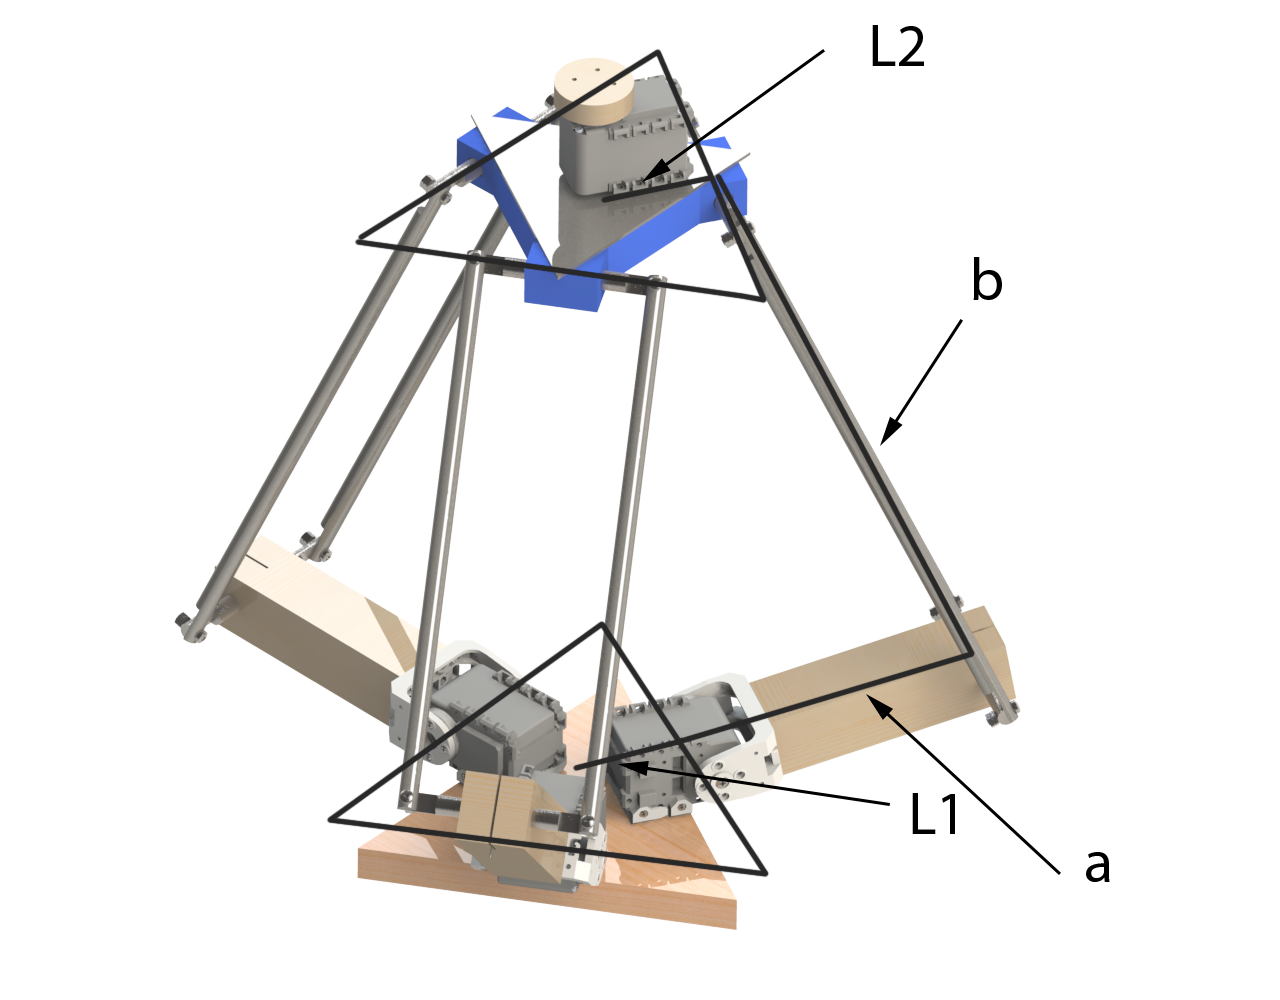
\includegraphics[width=12cm]{./imgComp/esquema_general}
\end{figure}

\begin{description}
\item[a] és la mida total del braç, des de l'eix del motor fins a l'eix de la connexió amb l'avantbraç.
\item[b] és la mida de tot l'avantbraç des de la connexió amb el braç fins a la unió amb la plataforma.
\item[L1] és la distància entre el centre de la base als eixos dels motors.
\item[L2] és la distància entre el centre de la plataforma a l'eix de connexió amb l'avantbraç.
\end{description}

\subsubsection{Canvis de base}
Com el càlcul de cada angle es independent de la resta, es poden fer canvis de base per poder fer-ho tot amb una sola funció a l'hora de programar. La base inicial \(\{x_0,y_0,z_0\}\) esta al centre de la base, amb la x en la direcció del motor 1. Les bases \(\{x_i,y_i,z_i\}\) que farem servir per calcular l'angle del motor \emph{i} estan posicionades al centre del eix de cada motor, i la seva x apunta en la direcció perpendicular al eix del motor.

\begin{figure}[h!]
\centering
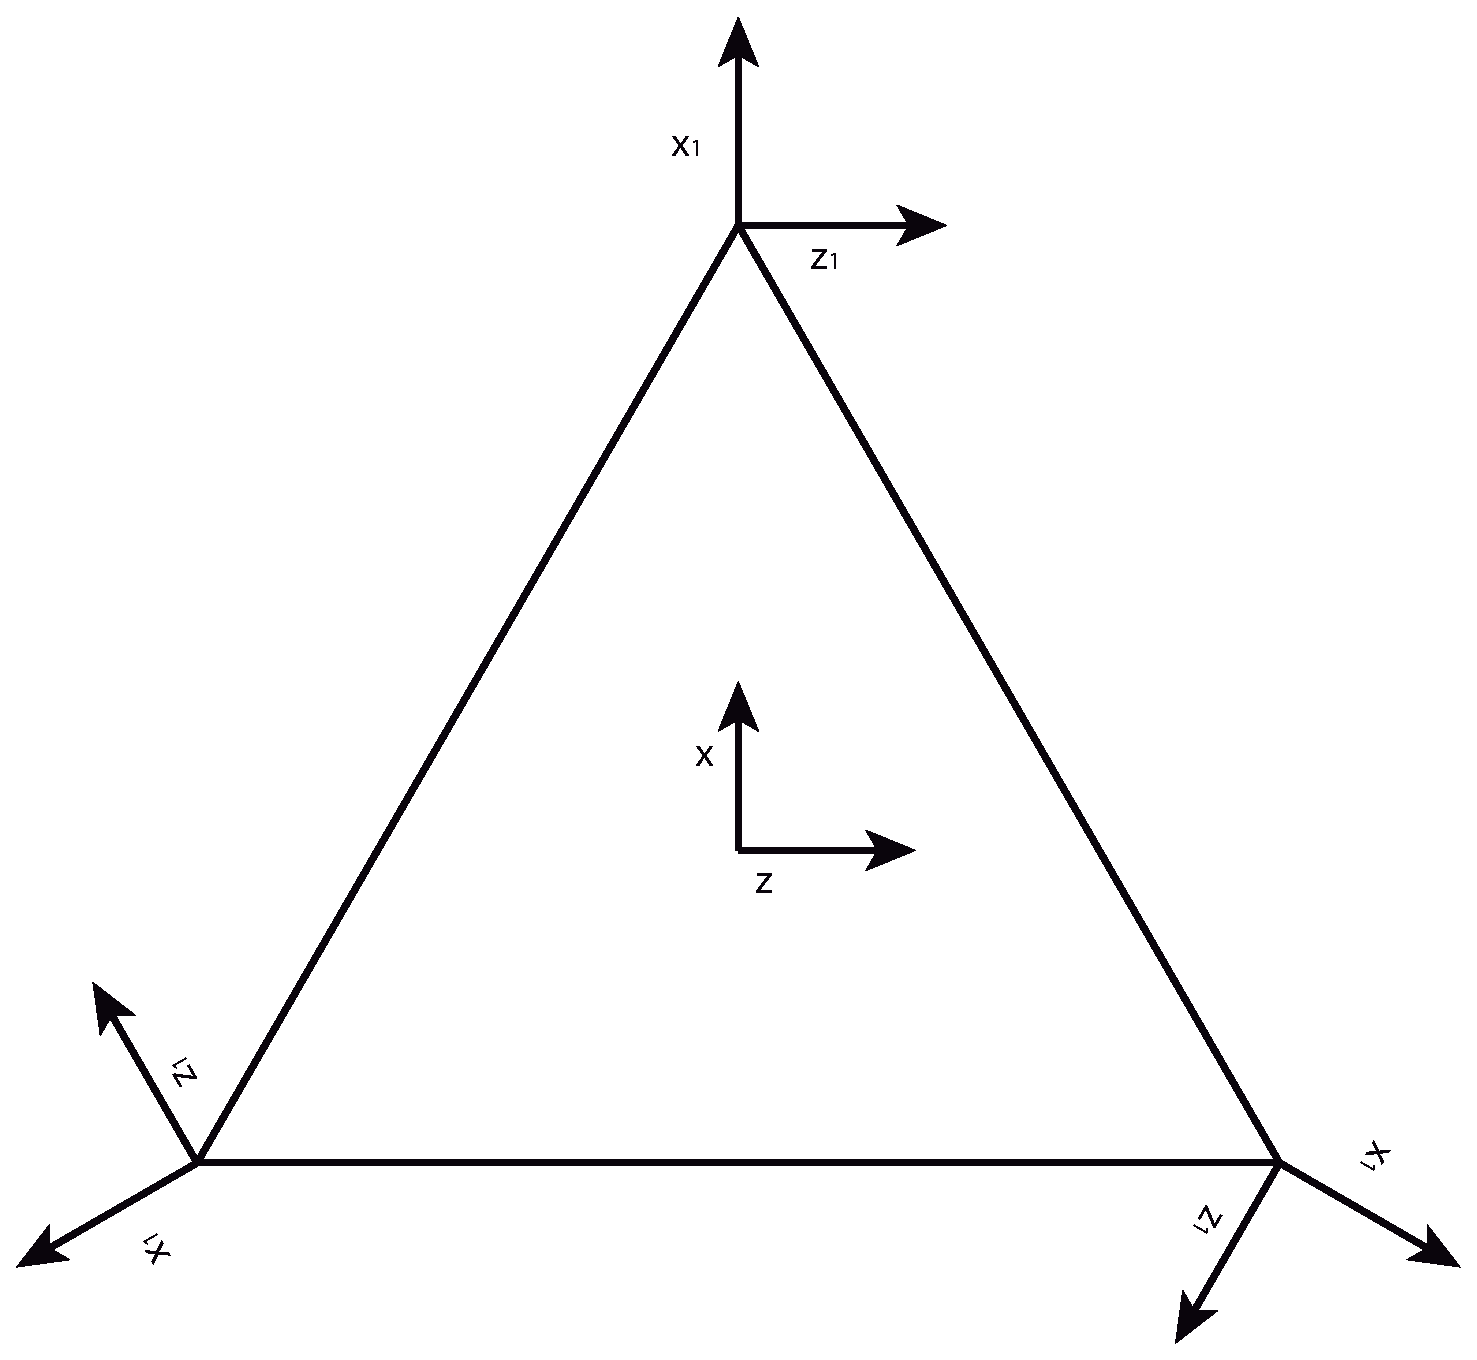
\includegraphics[width=8cm]{./sketch/canvi_base}
\end{figure}

\[\{x_1,y_1,z_1\}\=\{x_0+L2-L1,y_0,z_0\}\]
\[\{x_2,y_2,z_2\}\=\{z_0sin(60)-x_0cos(60)+L2-L1,y_0,-z_0cos(60)-x_0sin(60)\}\]
\[\{x_3,y_3,z_3\}\=\{-z_0sin(60)-x_0cos(60)+L2-L1,y_0,-z_0cos(60)+x_0sin(60)\}\]

\subsubsection{Càlcul d'un angle}

El motor només pot moure el final del braç en un cercle, gràcies a això es poden deduir dos formules:\[x^2+y^2=a^2 \quad \textrm{i} \quad z=0\]

\begin{figure}[h!]
\centering
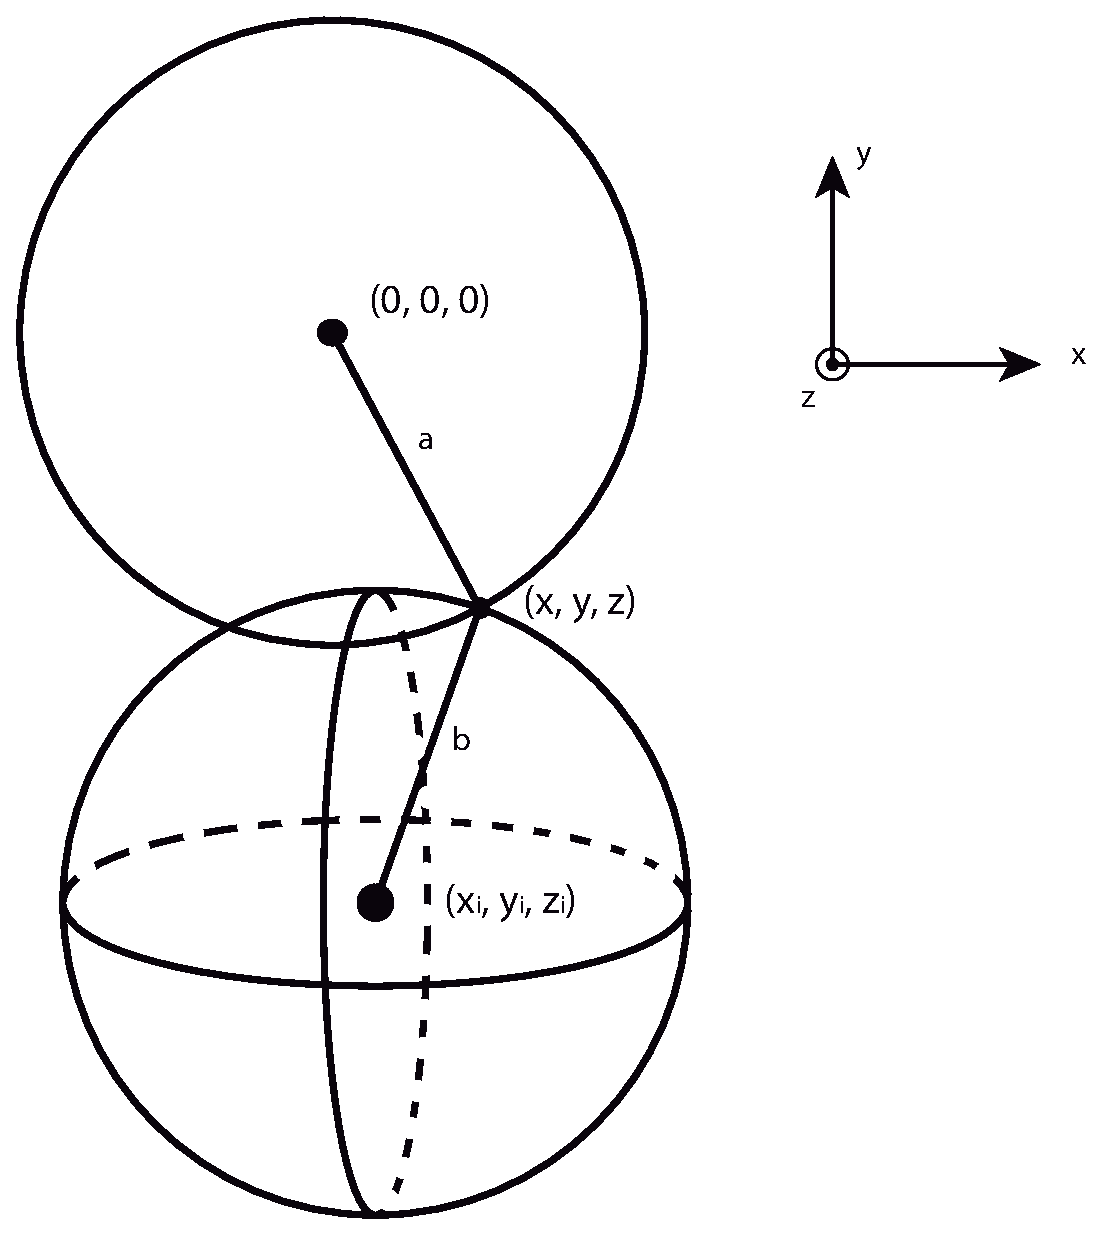
\includegraphics[width=8cm]{./sketch/calcul_angle}
\end{figure}

També es pot veure que, com ha d'estar connectat a la plataforma amb una distancia b mitjançant l'avantbraç, s'ha de complir la formula: \[(x-x_i)^2+(y-y_i)^2+(z-z_i)^2=b^2\]
Ara només cal resoldre el sistema d'equacions.

\[x^2-2xx_i+x_i^2+y^2-2yy_i+y_i^2+z_i^2=b^2\]
\[-2xx_i-2yy_i=b^2-a^2-x_i^2-y_i^2-z_i^2\equiv n\]
\[-2\sqrt{a^2-y^2}x_i=n+2yy_i\]
\[4a^2x_i^2-4y^2x_i^2=n^2+4yy_in+4y^2y_i^2\]
\[a^2x_i^2-y^2x_i^2=\frac{n^2}{4}+yy_in+y^2y_i^2\]
\[y^2(x_i^2+y_i^2)+y(y_in)+(\frac{n^2}{4}-a^2x_i^2)=0\]
\[y=\frac{-y_i\pm\sqrt{y_i^2n^2-4(x_i^2+y_i^2)(\frac{n^2}{4}-a^2x_i^2)}}{2(x_i^2+y_i^2)}\]
\[x=\pm\sqrt{a^2-y^2}\]
\[\textrm{Finalment, }\theta=atan(\frac{y}{x})\]

\subsection{Rang de treball}

Per calcular el rang de treball s'ha utilitzat la fórmula de l'apartat anterior  

\subsection{Implementació en C++}